\section{Multiple Learners}
Also called Ensemble Learning, is based on training many different learner/model and combine their result.

The general idea is that, if we use a baseline (single model) performances may be good, if we instead use bagging or voting (parallel) performances increases and if we use boosting (sequential) performance are even better.

\subsection{Voting}
Given a dataset $D$
\begin{enumerate}
    \item use $D$ to train a set of models $y_{m}(x)$, for $m = 1, \dots , M$
    \item make prediction with 
    \begin{equation}
        \begin{array}{lr}
             y_{voting}(x) = \sum w_{m}y_{m}(x) & \text{(regression)} \\
             y_{voting}(x) = \underset{c}{argmax}\sum w_{m}l(y_{m}(x)=c) & \text{weighted majority (classification)}
        \end{array}
    \end{equation}
\end{enumerate}
with the sum of $w_{m} = 1$, $l(e)=1$ if $e$ is true, 0 otherwise.\\
If we add a Non linear gating function $f$ depending on input, it is called \textbf{Mixture of experts}.\\
If we also try to learn the combination function $f$ it is called \textbf{Stakcing}.\\
\textbf{Cascading} learners are instead based on confidence threshold.\\
\\
\\
check coding scheme.\\
\\
\\
\subsection{Bagging}
Given a dataset $D$:
\begin{enumerate}
    \item generate M bootstrap data sets $D_{1} \dots D_{m}$, with $D_{i} \in D$.
    \item use each bootstrap data set $D_{m}$ to train a model $y_{m}(x)$, for each m.
    \item make predictions with a voting scheme
    \begin{equation}
        y_{bagging}(x) = \frac{1}{M} \sum y_{m}(x)
    \end{equation}
\end{enumerate}
\subsection{Boosting}
\subsubsection{general approach}
main points are:
\begin{itemize}
    \item Base classifiers (\textbf{weak learners}) trained \textbf{sequentially}
    \item Each classifier trained on weighted data
    \item Weights depend on performance of previous classifiers
    \item Points misclassified by previous classifiers are given greater weight. So that next models will classify better those points
    \item Predictions based on weighted majority of votes
\end{itemize}
\begin{figure}[H]
    \centering
    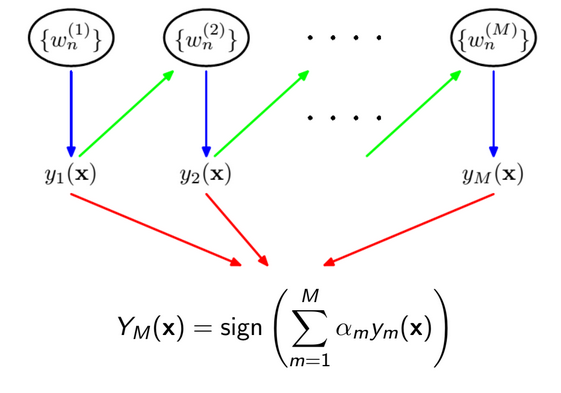
\includegraphics[width=15cm]{images/boosting/boosting.png}
    \label{fig:booting}
\end{figure}

\subsection{AdaBoost}
Given $D = \{(x_{1}, t_{1}), \dots, (x_{n}, t_{n})\}$, where $x_{n} \in X, t_{n} \in \{-1, +1\}$
\begin{enumerate}
    \item Initialize $w_{n}^{(m)}= 1/N,\ n=\, \dots, N$
    \item For $m=1, \dots, M$:
    \begin{itemize}
        \item Train a weak learner $y_{n}(x)$ my minimizing the weighted error function:
        \begin{equation}
            J_{m} = \sum_{n=1}*{N}w_{n}^{(m)}l(y_{m}(x_{n}) \neq t_{n})
        \end{equation}
        \item Evaluate: $\epsilon_{m} = \frac{\sum w_{n}^{(m)}l(y_{m}(x_{n}) \neq t_{n})}{\sum w_{n}^{(m)}}$ and $\alpha_{m}=\ln [\frac{1 - \epsilon_{m}}{\epsilon_{m}}]$
        \item Update the data weighting coefficients:
        \begin{equation}
            w_{n}^{(m+1)} = w_{n}^{(m)}exp[\alpha_{m}l(y_{m}(x_{n}\neq t_{n})]
        \end{equation}
    \end{itemize}
    \item Output the final classifier:
    \begin{equation}
        Y_{M}(x) = sign(\sum_{m=1}^{M}\alpha_{m}y_{m}(x))
    \end{equation}
\end{enumerate}
\begin{figure}[H]
    \centering
    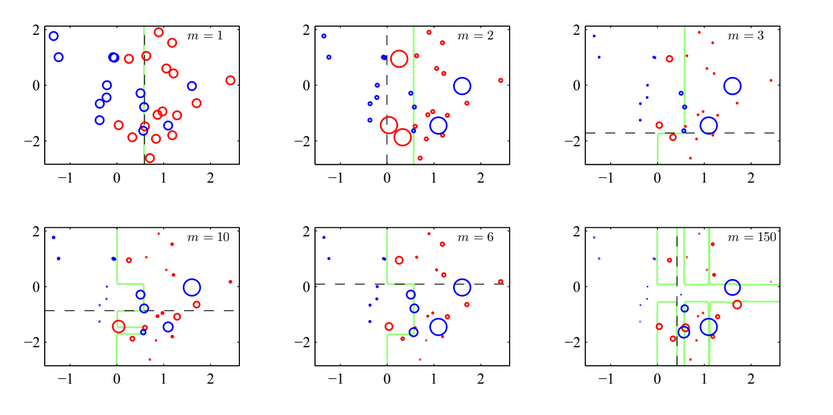
\includegraphics[width=15cm]{images/boosting/adaboost.png}
    \label{fig:adboost}
\end{figure}

\subsubsection{Exponential Error Minimization}
AdaBoosting can be explained as the sequential minimization of an exponential error function.\\
Consider the error function
\begin{equation}
    E = \sum_{n=1}^{N}exp[-t_{n}f_{M}(x_{n}],
\end{equation}
where $f_{M}$ is the final classifier
\begin{equation}
    f_{M}(x) = \frac{1}{2}\sum_{m=1}^{M}\alpha_{m}y_{m}(x),\ \ \ t_{n}\in \{-1, +1\}
\end{equation}
the goal is to minimize the error function $E$ w.r.t. $\alpha_{m}, y_{m}(x), m=1, \dots, M$

\textbf{Sequential minimization}, instead of minimizing $E$ \textit{globally}
\begin{itemize}
    \item assume $y_{1}(x), \dots, y_{M-1}(x)$ and $\alpha_{1}, \dots, \alpha_{M-1}$ fixed
    \item minimize w.r.t. $y_{M}(x)$ and $\alpha_{M}$.
\end{itemize}
Making $y_{M}(x)$ and $\alpha_{M}$ explicit we have:
\begin{equation}
    E=\sum_{n=1}^{N} exp[-t_{n}f_{M-1}(x_{n}) - \frac{1}{2}t_{n}\alpha_{M}y_{M}(x_{n}] = \sum w_{n}^{(M)}exp[-\frac{1}{2}t_{n}\alpha_{M}y_{M}(x_{n})]
\end{equation}
with $ w_{n}^{(M)} = exp[-t_{n}f_{M-1}(x_{n})]$ constant as we are optimizing w.r.t. $\alpha_{M}$ and $y_{M}(x)$

From sequential minimization we obtain $w_{n}^{(m+1)}$. Then we can predict with:
\begin{equation}
    sign(f_{M}(x)) = sign(\frac{1}{2}\sum \alpha_{m}y_{m}(x))
\end{equation}
which is equal to
\begin{equation}
    Y_{M}(x) =  sign(\sum \alpha_{m}y_{m}(x))
\end{equation}
thus providing that AdaBoost minimizes such error function

\subsubsection{AdaBoost: remarks}
Pros:
\begin{itemize}
    \item Fast and simple to implement
    \item no prior knowledge about base learners is required
    \item no parameters to tune
    \item can be combined with any method for finding best learners
    \item theoretical guarantees given sufficient data and base learners with moderate accuracy
\end{itemize}
Cons:
\begin{itemize}
    \item Performance depends on data and the base learners
    \item Sensitive to noise
\end{itemize}

